\documentclass[sigconf,nonacm]{acmart}

\settopmatter{printacmref=false, printccs=false, printfolios=true}
\setcopyright{none}
\acmConference{CS 567: 3D User Interfaces and Human-Centered Spatial AI}{Fall 2026}{Colorado State University}

\usepackage{xcolor}
\usepackage{graphicx}

\newcommand{\guide}[1]{{\color{gray}\itshape #1\par\medskip}}

\begin{document}

%% Title
\title{GARVIS-XR: Spatial Gestures and Visual Feedback for Immersive Scientific Visualization}
\subtitle{GARVIS: Spatial Intelligence Initiative}

%% Authors
\author{Ethan Sheffield}
\email{ethan.sheffield@colostate.edu}
\affiliation{%
  \institution{Colorado State University}
  \department{Department of Computer Science}
  \city{Fort Collins}
  \state{CO}
  \country{USA}}

\renewcommand{\shortauthors}{GARVIS: Spatial Intelligence Initiative}

%% Abstract
\begin{abstract}
Immersive scientific visualization can support the exploration of spatially complex data, but speech-driven interaction can become ambiguous when natural-language commands refer to specific objects within a three-dimensional setting. Although existing research has explored multimodal speech and gesture interaction and agentic interfaces for visualization, it is not yet well understood how spatial gestures and visual feedback can support reference resolution and error recovery in immersive scientific visualization. This project will extend NIST’s GARVIS with tracked spatial gesture input to select visualization objects and visual feedback indicating the object resolved as the target of a command. The system will be evaluated through a user study that compares speech-only input, speech-and-gesture input, and speech-and-gesture input with visual feedback using target selection accuracy, task completion time, error and correction rates, and subjective user measures. The results will provide insight into how spatial and visual interaction techniques can support more effective interaction with agentic scientific visualization systems. 
\end{abstract}

%% Keywords
\keywords{3D user interfaces; immersive visualization; speech-and-gesture 
interaction; spatial reference resolution; visual feedback; humanAI interaction}

\maketitle

%% Intro and Motivation
\section{Introduction and Motivation}

Immersive scientific visualization provides a platform for researchers and other technical professionals to interact with complex three-dimensional data while preserving spatial relationships that can be difficult to perceive through traditional desktop interfaces. However, interacting with these environments can require specialized interfaces and knowledge that create barriers for domain researchers. Natural-language interaction provides an alternative by allowing users to express visualization goals without directly manipulating every underlying operation. GARVIS demonstrates this approach through a speech-driven agentic interface for immersive scientific visualization \cite{su2025garvis}.

Despite these advantages, speech alone provides limited spatial information about what a user is referring to within a three-dimensional environment. A researcher may say “make that transparent” while several visualization objects are visible. The intended operation is clear, but the target is ambiguous. Recent work has demonstrated the potential of a multimodal approach, combining speech and gesture input, to reinforce user intent when using LLM-based interaction in general VR applications \cite{hu2025gesprompt}.

Existing research has explored multimodal speech-and-gesture interaction in immersive environments and agentic approaches to scientific visualization, but the intersection of these approaches for resolving ambiguous spatial references remains less understood. One open question is whether spatial gestures can reliably distinguish the intended visualization object when scenes contain overlapping objects, multiple visually similar elements, or dynamically changing data. Another is how visual feedback can help users recognize when an agent has resolved a command to an unintended target. Addressing these challenges requires considering both how users provide spatial information to an agent and how the agent communicates its interpretation back to the user.


%% Related Work
\section{Related Work}
\subsection{Natural and Multimodal Interaction in Immersive Visualization}

Prior work has explored speech input and multimodal interaction as alternatives to conventional interfaces for immersive visualization. Hombeck et al. demonstrated voice-based interaction for object orientation, visualization customization, and analytical tasks in medical VR~\cite{hombeck2024voice}. Su et al. investigated multimodal interaction techniques for immersive flow visualization and reported improved accuracy and interaction efficiency, along with reduced fatigue, when compared with conventional joystick-based interaction~\cite{su2021natural}. These studies demonstrate the potential for multimodal interaction to reduce the user burden of directly manipulating complex visualizations. 

\subsection{Speech, Gesture, and LLM-Based Interaction}

Recent work has begun combining speech and gesture with LLM-based systems to support more natural interaction in immersive environments. Hu et al. introduced GesPrompt, which combines gestures with speech to provide spatial and temporal information that may be difficult to communicate through language alone~\cite{hu2025gesprompt}. In GesPrompt, the language model identifies information that cannot be resolved from speech alone, while the gesture-processing component supplies spatial information associated with the spoken command~\cite{hu2025gesprompt}. This demonstrates how speech and gestures can complement one another when interacting with three-dimensional environments. Similarly, ParaView-MCP demonstrates the use of multimodal LLMs as agents for scientific visualization, allowing users to control ParaView through natural-language and visual inputs while enabling the agent to use viewport observations as visual feedback~\cite{liu2025paraview}. NIST’s GARVIS extends the ParaView-MCP paradigm through a speech-driven interface, demonstrating how natural-language commands can be used to control visualization tasks without requiring users to directly manipulate the underlying visualization tools~\cite{su2025garvis}. Together, these systems establish the feasibility of combining natural language, spatial information, and agentic AI. However, they leave open the question of how spatial gestures and feedback should be designed specifically for ambiguous references within immersive scientific visualizations.


%% Approach
\section{Approach}
\label{sec:approach}

This project will extend the GARVIS architecture with spatial gesture input and visual feedback to address ambiguous references in immersive scientific visualization. A tracked motion controller will provide a spatial pointing or raycast interaction that allows users to designate a visualization object while simultaneously issuing a natural-language command. For example, a user could point toward one of several objects and say, “make that transparent.” The speech input will specify the desired operation, while the gesture will provide the spatial information needed to identify the intended target. The selected object will then be visually highlighted or outlined to provide visual feedback indicating which visualization object the agent resolved as the target of the command. This extension will integrate with GARVIS’s existing ParaView-MCP tool pipeline rather than replace its speech, language-model, or visualization components.

The resulting system will enable comparison of three modality paradigms :  

\begin{enumerate}
\item Speech-only input
\item Speech and gesture input
\item Speech and gesture input with visual feedback
\end{enumerate}

This comparison will investigate whether spatial input reduces ambiguity in natural-language visualization commands and whether visual feedback helps users recognize the agent’s interpretation before or during execution. 


%% System Vision and Tech
\section{System Vision and Technology}

The completed system will allow a user wearing a Meta Quest 2 or Quest 3, or using a CAVE system, to interact with ParaView visualizations using speech and a tracked motion controller. The user will point toward a visualization object while issuing a natural-language command, after which the selected object will be highlighted or outlined to provide visual feedback. 

This project will extend the existing Garvis stack, including Garvis.py, WhisperLiveKit, Claude, ParaView-MCP, and ParaView, as shown in Figure~\ref{fig:ArchitectureDiagram}.

\begin{figure}[h]
  \centering
  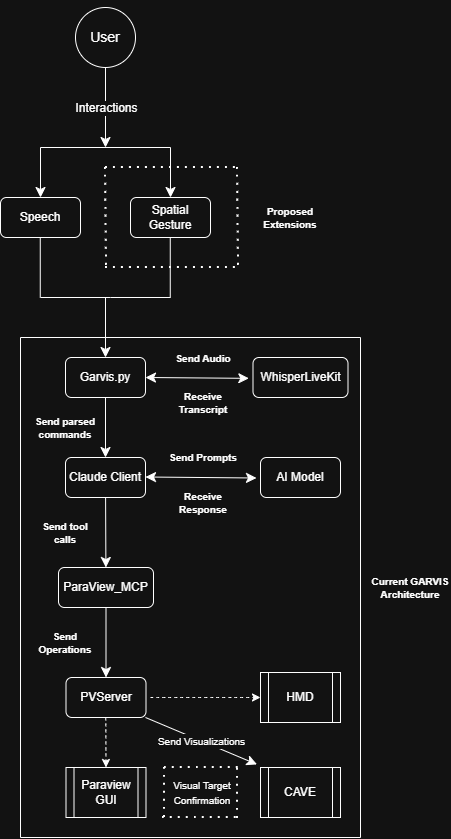
\includegraphics[width=\columnwidth]{figures/ArchitectureDiagram.png}
  \caption{The proposed project’s extended GARVIS architecture incorporating spatial gesture input and visual target feedback.}
  \label{fig:ArchitectureDiagram}
\end{figure}

The proposed work will add tracked controller input and visual target feedback while preserving the existing speech-driven agentic pipeline, as shown in Figure~\ref{fig:InteractionDiagram}. The demonstration will show the three interaction conditions described in Section~\ref{sec:approach}. 

\begin{figure}[h]
  \centering
  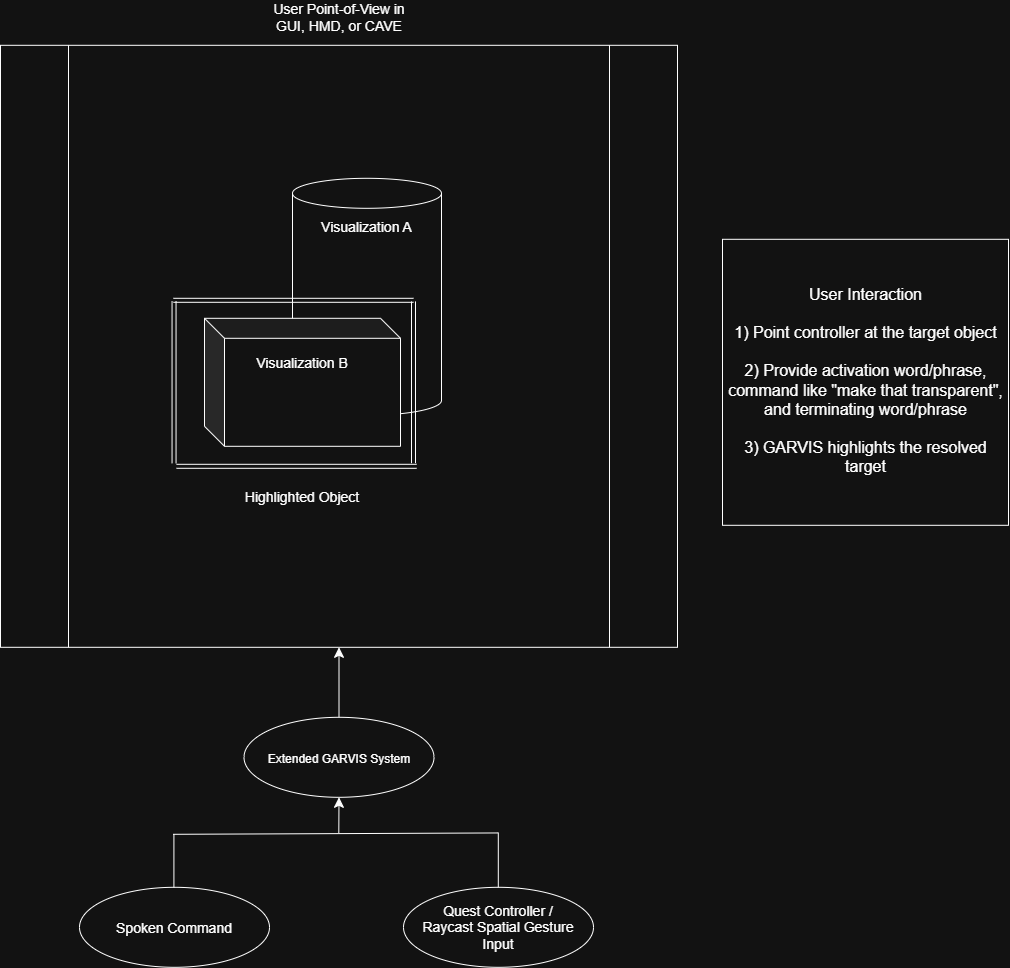
\includegraphics[width=\columnwidth]{figures/InteractionDiagram.png}
  \caption{ A mockup of the proposed multimodal GARVIS interaction, showing speech and spatial gesture input with visual feedback of the resolved target.}
  \label{fig:InteractionDiagram}
\end{figure}


%% Evaluation Plan
\section{Evaluation Plan}
\subsection{Research Questions}

\textbf{RQ1:} How does the addition of spatial gesture input affect users' ability to specify and resolve references to visualization objects in immersive scientific visualization, especially when verbal commands are ambiguous?
\textbf{RQ2:} How does visual feedback affect users' ability to recognize and recover from the agent's interpretation of their commands?

\subsection{Independent Variable}
The primary independent variable will be interaction technique, with three conditions:

\begin{enumerate}
\item \textbf{Speech-only:} Users issue natural-language commands without spatial gesture input or visual target feedback.
\item \textbf{Speech + Gesture:} Users issue natural-language commands while using a spatial pointing gesture to identify the intended visualization object. 
\item \textbf{Speech + Gesture + Visual Feedback:} Users issue natural-language commands with spatial pointing while the system provides visual feedback indicating the visualization object resolved as the target of the command.
\end{enumerate}

This progression isolates the contribution of each interaction modality. Speech establishes the baseline, gesture adds spatial information for reference resolution, and visual feedback adds information about how the agent interpreted the combined input.

\subsection{Dependent Variables and Measures}
The evaluation will measure target selection accuracy, task completion time, error and correction rates, and subjective user experience.

\begin{itemize}
\item \textbf{Target selection accuracy:} Whether the system correctly identifies the visualization object intended by the participant.
\item \textbf{Task completion time:} The time required for a participant to successfully complete each visualization task.
\item \textbf{Error rate:} The percentage of trials in which the system selects or interprets an unintended target.
\item\textbf{Correction rate:} The percentage of system errors that participants recognize and successfully correct.
\item \textbf{User confidence:} Participants' reported confidence that the system correctly understood their intended target and command.
\item \textbf{Workload and usability:} Subjective measures collected to assess the perceived effort and usability of each interaction technique.
\end{itemize}

The primary dependent variables will be target selection accuracy, task completion time, and error and correction rates, while subjective measures will provide additional information about participants' perceptions of the interaction techniques.

\subsection{Task}
Participants will complete immersive visualization tasks using natural-language commands directed at specific visualization objects. Tasks will include both unambiguous and intentionally ambiguous commands, such as changing the color or transparency of one object among several visible objects. Performance across the three interaction conditions will be compared to evaluate reference resolution and error recovery.

\subsection{Participants and IRB}
The study will recruit participants with basic familiarity with VR interaction. An IRB submission and approval will be required before collecting human-subject data. Participant count, experiment protocol, and statistical analysis will be finalized as the prototype and project are further developed.


%% Deliverables
\section{Deliverables}
\label{sec:deliverables}

\begin{itemize}
\item \textbf{GARVIS-XR Implementation:} A working immersive visualization system extending GARVIS with spatial gesture input and visual target feedback, integrated with the existing ParaView-MCP pipeline and deployable in the target VR environment.
\item \textbf{Evaluation Data and Results:} A completed user study comparing the three interaction conditions, including logged task performance, target selection accuracy, completion times, error/correction rates, and subjective user feedback, along with the resulting analysis
\item \textbf{Research Paper and Demonstration Materials:} A completed research paper documenting the motivation, related work, system implementation, experimental methodology, results, and findings. The research paper will be accompanied by videos demonstrating the implemented interaction techniques and evaluation setup.
\end{itemize}


%% Conclusion
\section{Conclusion}

This project will extend GARVIS into an immersive multimodal visualization system by integrating spatial gesture input and visual feedback with its existing speech-driven interface. The project will investigate whether these additions support the resolution of ambiguous spatial references and help users recognize and recover from incorrect agent interpretations. By the end of the project, the class should expect to see a working GARVIS-XR implementation, results from a user evaluation, and a completed research paper documenting the system and findings. 


%% AI Disclaimer
\section*{Use of AI}

LLMs were used during the development of this project proposal to assist in identifying relevant research resources and to help assess whether the proposed research direction appeared to address an existing gap in the literature. AI-generated suggestions were used as a starting point for further investigation, and sources and research claims were independently reviewed and verified. 


%% References
\bibliographystyle{ACM-Reference-Format}
\bibliography{references}

\end{document}